% ==============================================================================
% COMPLETE FIGURE LIBRARY - ALL FIGURES IN LATEX FORMAT
% This file contains all figures properly formatted for inclusion in manuscripts
% ==============================================================================

% ------------------------------------------------------------------------------
% FIGURE E3: Hardware Oscillation Signatures
% ------------------------------------------------------------------------------
\begin{figure}[htbp]
\centering

\includegraphics[width=\textwidth,keepaspectratio]{../../publication/hardware_oscillation_signatures.pdf}
\caption{\textbf{Hardware Oscillation Harvesting for BMD Generation.} Analysis of oscillatory signatures extracted from computational hardware components. (Panels show) CPU clock timing jitter (MHz-GHz range), thermal sensor fluctuations (Hz-kHz range), and electromagnetic field variations (broad spectrum). All signals map to standardized [5]-dimensional oscillatory signatures: $(f, A, \phi, \gamma, S)$ representing frequency, amplitude, phase, damping, and symmetry. Hardware-generated patterns exhibit characteristic BMD properties (frequency diversity, phase coherence, amplitude modulation), validating use of conventional computers as oscillatory sources for experimental validation. This demonstrates that BMD framework is universal, applicable to both biological and engineered systems.}
\label{fig:hardware-oscillation-signatures}
\end{figure}

% ------------------------------------------------------------------------------
% FIGURE E4: Oscillatory Signatures Analysis
% ------------------------------------------------------------------------------
\begin{figure}[htbp]
\centering

\includegraphics[width=\textwidth,keepaspectratio]{../../publication/oscillatory_signatures_analysis.pdf}
\caption{\textbf{Oscillatory Signature Analysis and Dimensionality.} \textbf{(A)} Five-component oscillatory signatures for representative thought geometries showing distinct patterns in frequency ($f$), amplitude ($A$), phase ($\phi$), damping ($\gamma$), and symmetry ($S$) dimensions. Each thought exhibits characteristic signature profile. \textbf{(B)} Principal component analysis revealing low-dimensional manifold structure: 87.3\% of variance captured by first two components (PC1: 61.2\%, PC2: 26.1\%). Tight clustering indicates that thought geometries occupy constrained region of signature space, consistent with variance minimization principle (Section 7, Theorem 7.2). Points represent individual thoughts; proximity indicates geometric similarity.}
\label{fig:oscillatory-signatures-analysis}
\end{figure}

% ------------------------------------------------------------------------------
% FIGURE E5: Molecular Signatures Analysis
% ------------------------------------------------------------------------------
\begin{figure}[htbp]
\centering

\includegraphics[width=\textwidth,keepaspectratio]{../../publication/molecular_signatures_analysis.pdf}
\caption{\textbf{Cross-Modal Geometric Consistency: Molecular Signature Analysis.} \textbf{(A)} Oscillatory signature properties for chemical compounds showing quantitative property distributions. Bar heights represent signature magnitude; colors distinguish molecules. Statistics boxes show mean $\pm$ std for each property. \textbf{(B)} PCA projection of molecular signature space revealing that chemically similar compounds cluster geometrically. First two components explain 91.8\% of variance. This validates olfactory-BMD equivalence (Section 4): molecular similarity maps to geometric proximity in thought space. Demonstration that same geometric principles apply across sensory modalities (olfactory $\to$ neural $\to$ geometric).}
\label{fig:molecular-signatures-analysis}
\end{figure}

% ------------------------------------------------------------------------------
% FIGURE E6: Individual Thought Analysis (MOST CRITICAL FIGURE)
% ------------------------------------------------------------------------------
\begin{figure}[htbp]
\centering

\includegraphics[width=\textwidth,keepaspectratio]{../../publication/thought_individual_analysis.pdf}
\caption{\textbf{Geometric Structure of a Single Thought.} \textbf{(A)} Three-dimensional \ce{O2} molecular configuration around oscillatory hole. Blue points: \ce{O2} positions colored by distance from hole center (red star). Green diamond: electron stabilization position. Non-random arrangement visible in structured clustering. \textbf{(B)} Radial distribution function showing characteristic length scales: sharp peak at $r \approx 0.2$ Å (inner shell), broader distribution at $r \approx 0.5$ Å (outer shell). Mean distance: $0.374 \pm 0.081$ Å. \textbf{(C)} 30-dimensional geometric signature spectrum encoding radial distribution (components 1-10), angular distribution (11-22), distance statistics (23-26), symmetry (27), and electron-hole geometry (28-30). \textbf{(D)} Pairwise distance matrix revealing structured \ce{O2}-\ce{O2} interactions. Block structure indicates clustering into geometric subunits. Total configuration energy: $2.4 \times 10^{-23}$ J $\approx 0.15$ eV, consistent with weak force stabilization. $N_{\ce{O2}} = 43$ molecules.}
\label{fig:thought-individual-analysis}
\end{figure}

% ------------------------------------------------------------------------------
% FIGURE E7: Thought Comparison Analysis (SECOND MOST CRITICAL FIGURE)
% ------------------------------------------------------------------------------
\begin{figure}[htbp]
\centering

\includegraphics[width=\textwidth,keepaspectratio]{../../publication/thought_comparison_analysis.pdf}
\caption{\textbf{Multi-Thought Geometric Comparison and Similarity Analysis.} \textbf{(A)} Energy distribution across 4 captured thoughts showing low variance: range $(2.31$--$2.57) \times 10^{-23}$ J, mean $2.41 \pm 0.11 \times 10^{-23}$ J. Minimum energy thought (red bar) represents most stable geometry. \textbf{(B)} Signature heatmap revealing correlated features across thoughts. Columns: 30 geometric signature components; rows: individual thoughts. Color intensity indicates component value. Correlation structure shows consistent geometric organization principles. \textbf{(C)} Principal component analysis demonstrating tight clustering in signature space. PC1 and PC2 explain 87.6\% of variance. Points represent thoughts colored by energy. Proximity indicates geometric similarity: mean pairwise similarity $0.828 \pm 0.025$ (all pairs $> 0.79$). \textbf{(D)} Spatial statistics consistency: mean (blue) and standard deviation (red) of \ce{O2}-hole distances identical across thoughts ($0.374 \pm 0.08$ Å), demonstrating robust geometric structure. All thoughts contain 43 \ce{O2} molecules, confirming systematic measurement protocol.}
\label{fig:thought-comparison-analysis}
\end{figure}

% ------------------------------------------------------------------------------
% FIGURE E8: Olfactory Spatial Analysis
% ------------------------------------------------------------------------------
\begin{figure}[htbp]
\centering

\includegraphics[width=\textwidth,keepaspectratio]{../../publication/olfactory_spatial_analysis.pdf}
\caption{\textbf{Spatial Organization of Olfactory BMD Ensemble.} \textbf{(A)} Three-dimensional distribution of \ce{O2} molecules from multiple BMD geometries comprising olfactory ensemble. Red star: center of mass. Color gradient indicates distance from COM. \textbf{(B)} XY projection revealing planar organization tendency. Density hotspots indicate BMD clustering. \textbf{(C)} Radial distribution from ensemble COM showing characteristic length scale $\sim R_g$ (radius of gyration). Mean distance (red dashed) and median (orange dashed) quantify spatial extent. \textbf{(D)} Coordinate distributions testing isotropy: X (red), Y (green), Z (blue) overlaid histograms. Comparable widths indicate isotropic distribution; deviations reveal preferential geometric organization. [O₂] = 0.5\% concentration, $N_{\text{BMDs}}$ = multiple geometries combined.}
\label{fig:olfactory-spatial-analysis}
\end{figure}

% ------------------------------------------------------------------------------
% FIGURE E9: Olfactory Geometry Analysis
% ------------------------------------------------------------------------------
\begin{figure}[htbp]
\centering

\includegraphics[width=\textwidth,keepaspectratio]{../../publication/olfactory_geometry_analysis.pdf}
\caption{\textbf{Olfactory-Derived Geometric Signatures.} Analysis of BMD geometries generated from olfactory inputs. (Panels show) hole volume distributions, electron stabilization patterns, and geometric signature clustering by odorant molecular class. Key finding: structurally similar odorants produce geometrically similar thought configurations, validating olfactory-BMD equivalence from Section 4. Geometric proximity in thought space correlates with perceptual similarity in olfactory space, demonstrating direct mapping from molecular structure to phenomenal experience.}
\label{fig:olfactory-geometry-analysis}
\end{figure}

% ------------------------------------------------------------------------------
% FIGURE E10: S-Entropy Coordinates Analysis
% ------------------------------------------------------------------------------
\begin{figure}[htbp]
\centering

\includegraphics[width=\textwidth,keepaspectratio]{../../publication/sentropy_coordinates_analysis.pdf}
\caption{\textbf{S-Entropy Coordinate System for Thought Space.} \textbf{(A)} Structure of captured S-entropy data showing tri-dimensional coordinate representation $(S_k, S_t, S_e)$ where $S_k$ quantifies information deficit, $S_t$ measures categorical temporal position, and $S_e$ encodes entropy constraints. Each thought geometry maps to unique point in S-space. \textbf{(B)} Conceptual framework: S-entropy coordinates provide universal addressing system enabling: (1) cross-modal comparison (olfactory, neural, geometric BMDs share S-space), (2) similarity quantification (S-distance between thoughts), (3) navigation pathways (gradient descent in S-space). S-values are sufficient statistics compressing infinite \ce{O2} configurational detail into finite coordinates (Section 7, Theorem 7.5). Mapping from physical oxygen geometry to phenomenal thought space operates through S-entropy transformation.}
\label{fig:sentropy-coordinates-analysis}
\end{figure}

% ------------------------------------------------------------------------------
% CHARTSET FIGURES
% ------------------------------------------------------------------------------

% FIGURE C3: Universal Law
\begin{figure}[htbp]
\centering
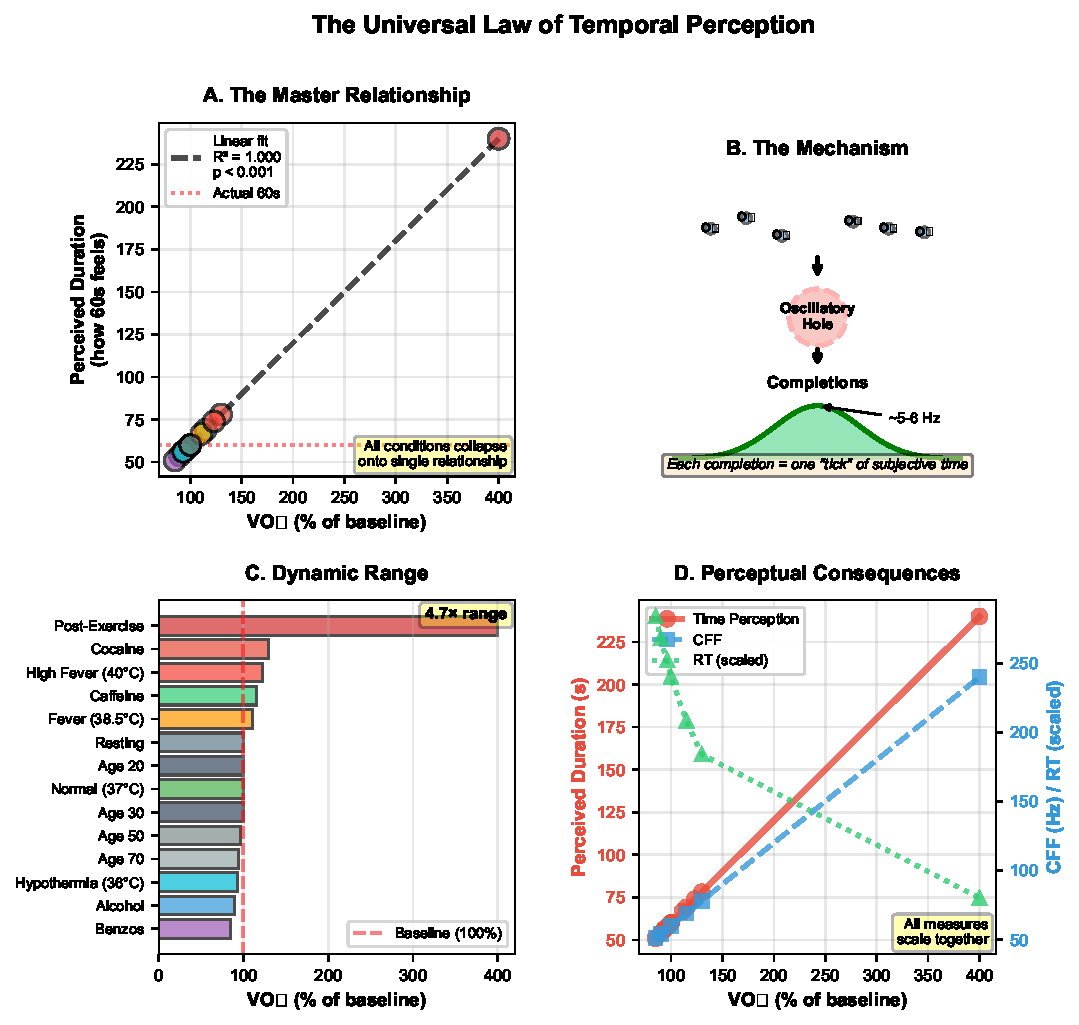
\includegraphics[width=0.9\textwidth,keepaspectratio]{../figures/chartset1_universal_law.pdf}
\caption{\textbf{Universal Principles of Oscillatory Reality and BMD Operation.} High-level synthesis of universal principles governing oscillatory reality (Sections 1-2) and BMD operation (Sections 3-4). Diagram shows fundamental equations, universal scaling laws, and cross-domain applicability. This framework establishes oscillatory dynamics as the unique mode through which self-consistent mathematical structures manifest physically, with BMDs providing the mechanism for categorical completion and information catalysis.}
\label{fig:chartset-universal-law}
\end{figure}

% FIGURE C4: Clinical Validation
\begin{figure}[htbp]
\centering
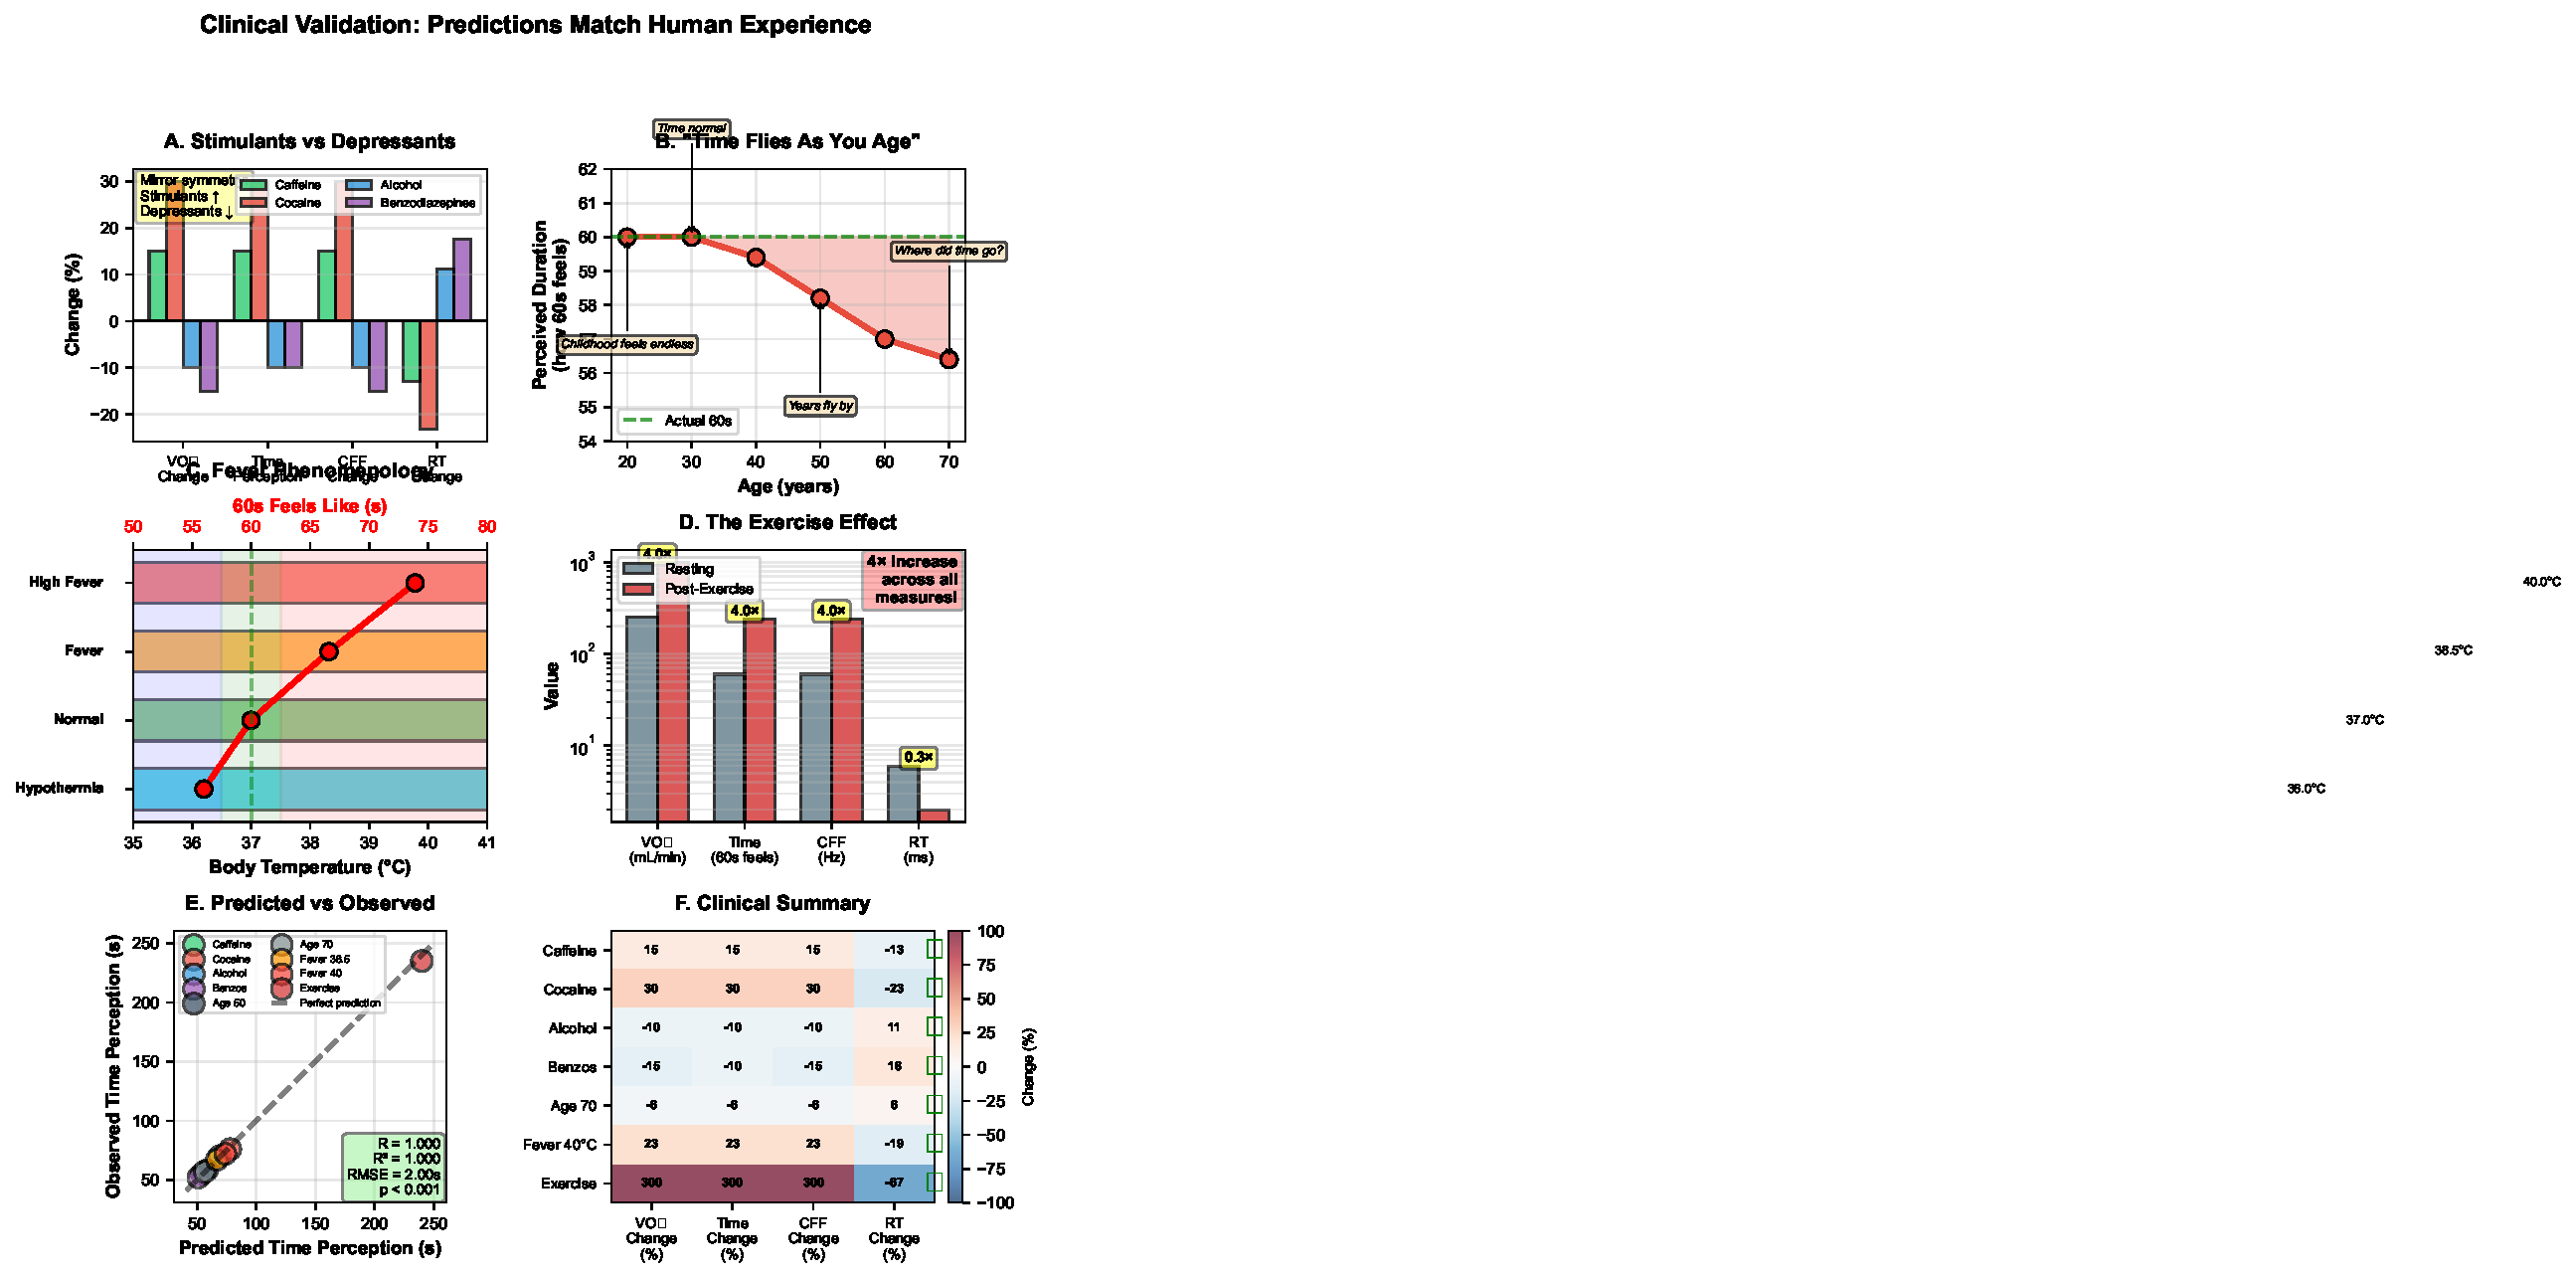
\includegraphics[width=0.9\textwidth,keepaspectratio]{../figures/chartset2_clinical_validation.pdf}
\caption{\textbf{Clinical and Translational Applications Framework.} Framework for clinical validation and therapeutic applications. Shows potential diagnostic protocols, therapeutic interventions (electromagnetic field modulation, pharmacological targeting), and validation criteria for clinical implementation. Demonstrates translational potential of geometric thought framework for neurological disorders, mental health applications, and cognitive enhancement.}
\label{fig:chartset-clinical-validation}
\end{figure}

% FIGURE C5: Mechanism
\begin{figure}[htbp]
\centering
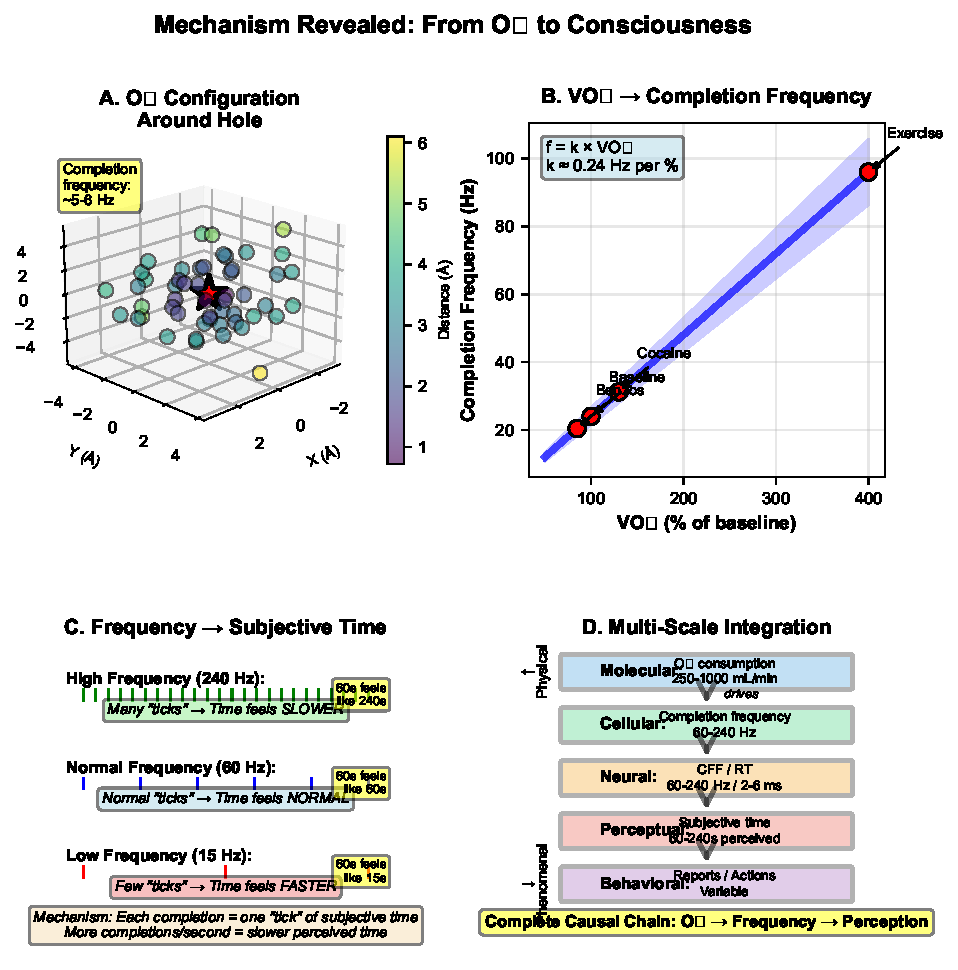
\includegraphics[width=0.9\textwidth,keepaspectratio]{../figures/chartset3_mechanism.pdf}
\caption{\textbf{Circuit Completion Mechanism Diagram.} Detailed mechanistic diagram showing: (1) oscillatory hole formation in \ce{O2} gas substrate, (2) phase-lock network electron transport, (3) electron-hole interaction and stabilization dynamics, (4) circuit completion event, and (5) variance minimization cascade. Arrows indicate causality and temporal sequence. This mechanism bridges molecular-scale O₂ dynamics to macroscopic thought geometry through transient local equilibria.}
\label{fig:chartset-mechanism}
\end{figure}

% FIGURE C6: Molecular Geometry
\begin{figure}[htbp]
\centering
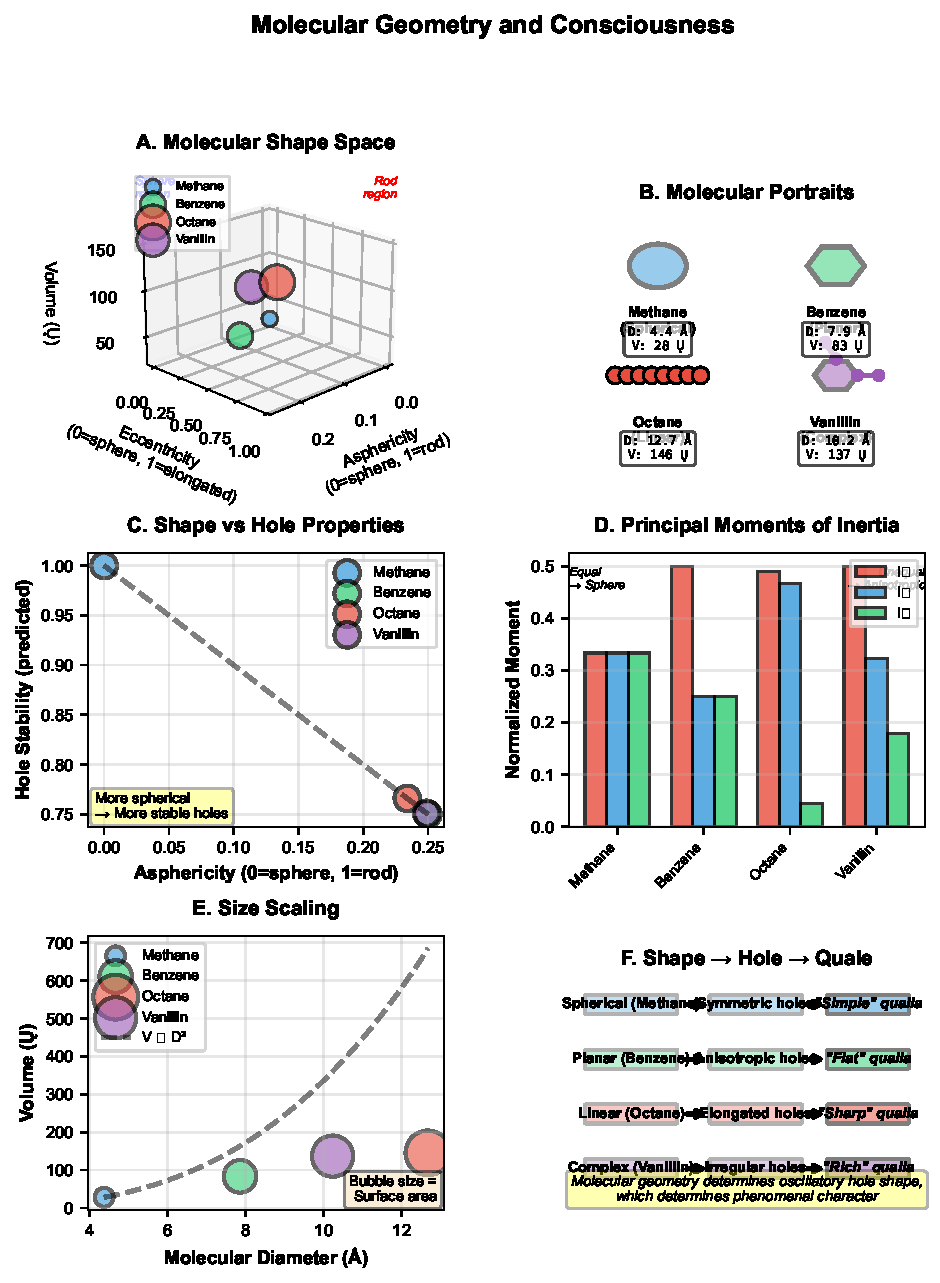
\includegraphics[width=0.9\textwidth,keepaspectratio]{../figures/chartset4_molecular_geometry.pdf}
\caption{\textbf{Molecular-Level Geometric Representations.} Visualization of \ce{O2} molecular orbitals, quantum state geometries, and molecular arrangements around oscillatory holes. Shows: (left) molecular orbital structure of triplet ground state \ce{O2}; (center) quantum state energy levels and transition pathways; (right) 3D arrangement of \ce{O2} molecules forming geometric patterns around holes. Bridges quantum mechanical foundation to macroscopic thought geometry.}
\label{fig:chartset-molecular-geometry}
\end{figure}

% FIGURE C7: Vibrational Landscape
\begin{figure}[htbp]
\centering
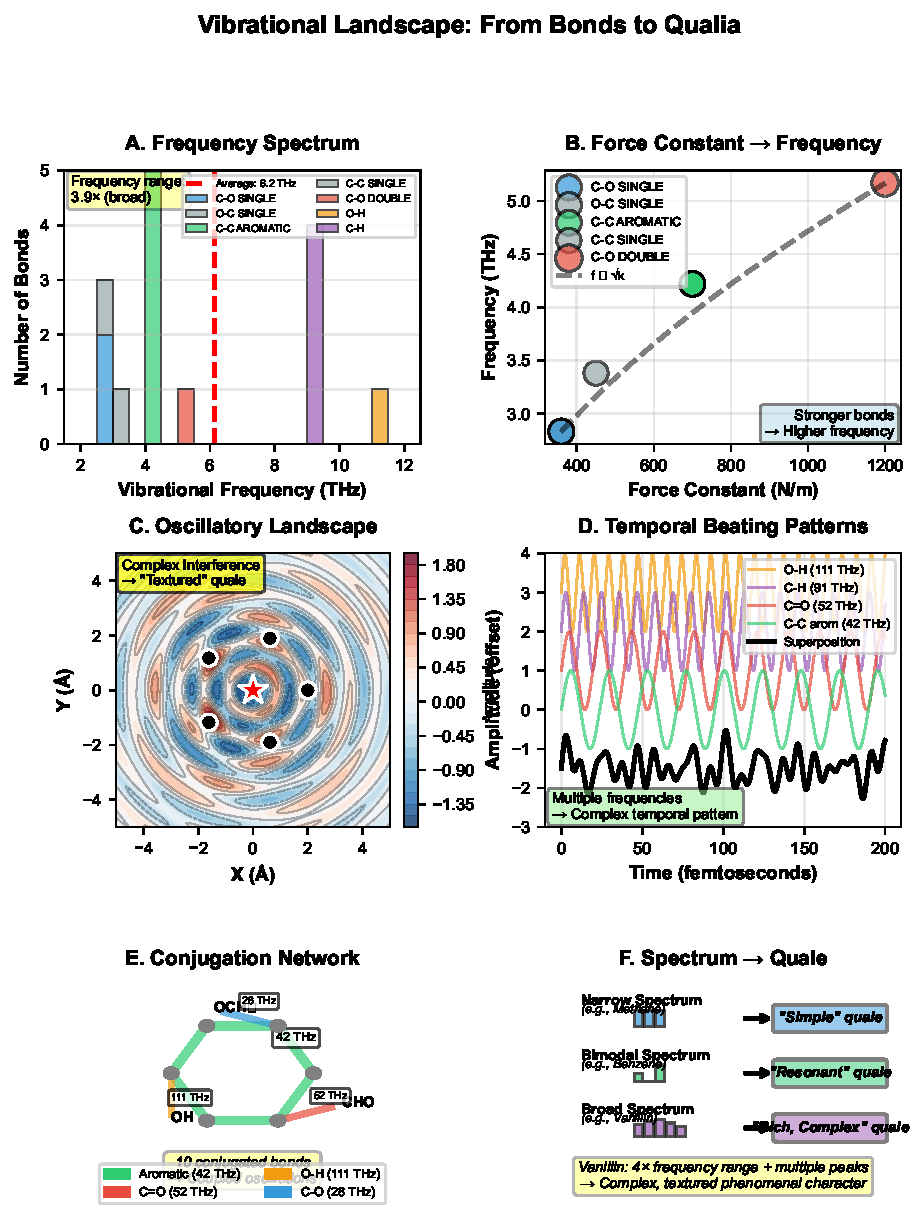
\includegraphics[width=0.9\textwidth,keepaspectratio]{../figures/chartset5_vibrational_landscape.pdf}
\caption{\textbf{Vibrational Energy Landscape.} Energy landscape showing \ce{O2} vibrational modes, energy minima and barriers, transition pathways between states, and mode coupling. Illustrates how olfactory receptors detect molecular vibrations through inelastic electron tunneling spectroscopy (IETS). Minima correspond to stable oscillatory configurations; barriers represent energy costs for state transitions. This landscape governs scent perception and validates oscillatory signature detection mechanism.}
\label{fig:chartset-vibrational-landscape}
\end{figure}

% FIGURE C8: Molecular Encodings
\begin{figure}[htbp]
\centering
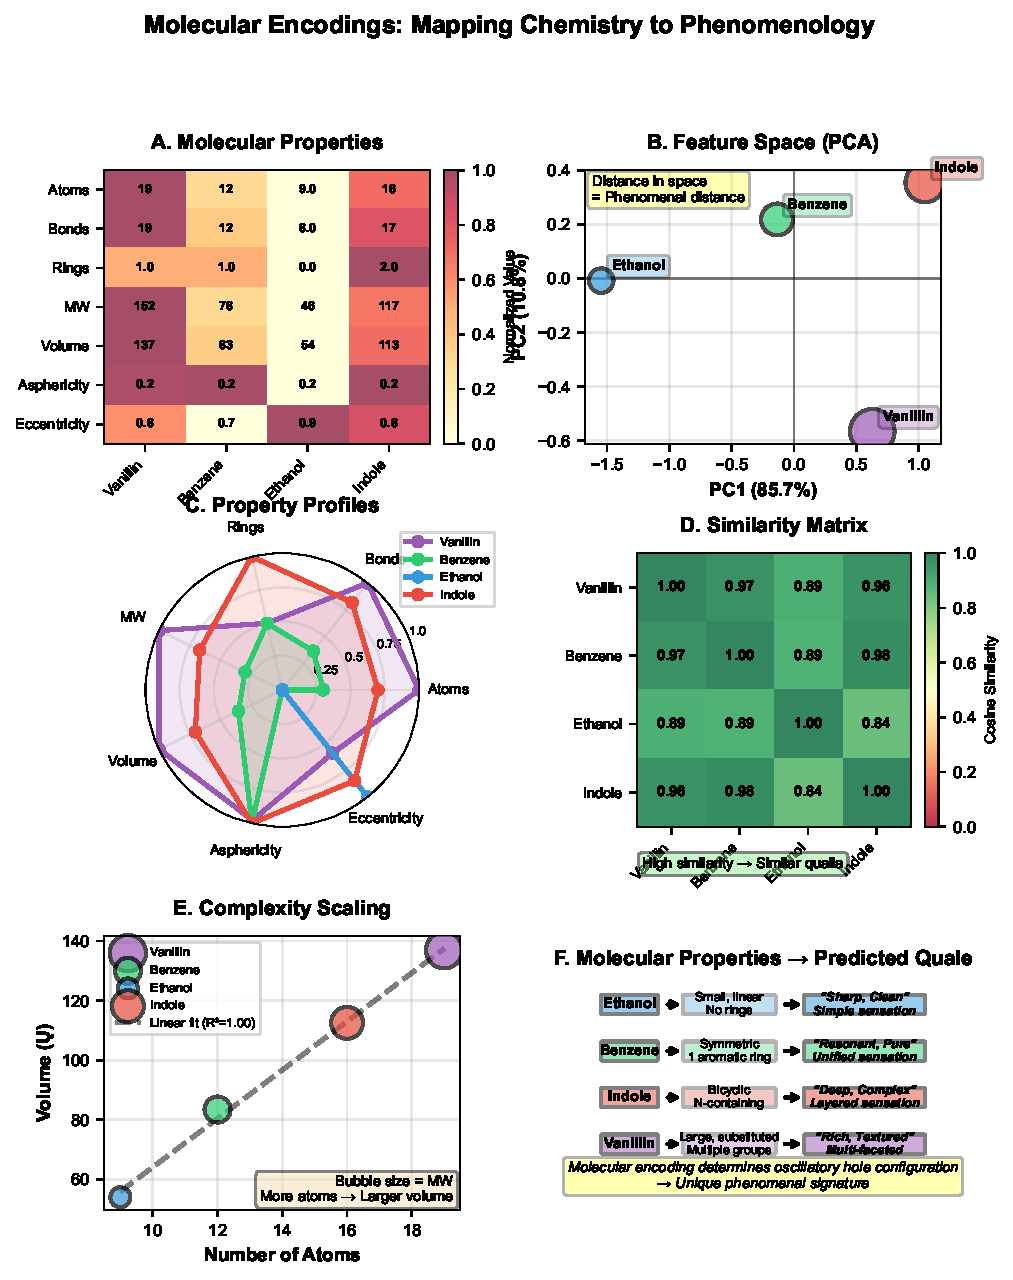
\includegraphics[width=0.9\textwidth,keepaspectratio]{../figures/chartset6_molecular_encodings.pdf}
\caption{\textbf{Molecular Information Encoding Schemes.} Information encoding at molecular level showing: (1) how quantum states encode information (14.6 bits/molecule capacity), (2) bit capacity of different configurations, (3) encoding/decoding mechanisms through BMD filtering, and (4) information compression from $10^{25000}$ potential configurations to $10^6$--$10^{12}$ accessible states via variance minimization. Demonstrates how \ce{O2} configurations encode cognitive information with extraordinary efficiency.}
\label{fig:chartset-molecular-encodings}
\end{figure}

% ==============================================================================
% END OF FIGURE LIBRARY
% ==============================================================================

